\section{Offline Computation}
The offline computation of selective decoding retrieves the dependencies by partially decoding a video. It is essential to understand various dependencies in order to comprehend offline computation.

For all subsequent disscussions in this paper, we assume the video is in YCbCr420 color space, which means a macroblock contains four luminance blocks and two chrominance blocks.  

\subsection{Dependencies}
Two categories of dependencies can be identified, namely intra-VOP dependency and inter-VOP dependency. Dependencies are the reason why some macroblocks outside of ROI need to be decoded. By saving certain information at offline computation, we can reduce the dependencies and improve the efficiency of selective decoding. Below we analyze the dependencies and introduce the methods to reduce them. 

\subsubsection{Intra-VOP Dependency}
Intra-VOP dependency refers to the dependencies among macroblocks within a single VOP. There are two sources of intra-VOP dependency, including DC\&AC Prediction and MV coding. 

DC\&AC Prediction is performed for I-macroblock when the header field short\_video\_header is set to '0' in MPEG4 SP bistream. DC\&AC Prediction decoding consists of two steps, reference block selection and prediction decoding. The reference block selection step can be illustrated by figure below,
\begin{figure}
\centering 
%\vspace{2.5cm}
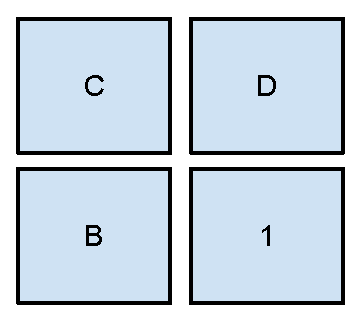
\includegraphics[height=1.5cm]{2.eps}
\caption{DC\&AC Prediction Reference Block Selection}
\end{figure}
There are two candidate reference blocks for each block, the immediate left block and the immediate upper block. In addition, the upper left block is also needed in order to determine the reference block. To determine the reference block for block 1 in figure above, the following rule is applied,
%\begin{verbatim} 
{\tt \\if (|F(B)[0][0] - F(C)[0][0]| < |F(C)[0][0] - F(D)[0][0]|)\\
\indent predict from block D \\
else  \\
\indent predict from block B \\} 
%\end{verbatim}
Note that F(B)[0][0], F(C)[0][0] and F(D)[0][0] refer to inverse quantized DC value of block B, C and D respectively. The selection rule indicates one block is dependent on three neighboring blocks. Once the reference block is selected, prediction coding can be carried out, where the decoding block depends only on the selected reference block.

Two out of three blocks are only needed to determine the prediction direction, which is either up or left. A single bit is enough to record this information, with '0' indicating up and '1' referring to left. This reduces the dependency for a block from three to one.

MVs of P-VOP is differentially coded, which is the other source of intra-VOP dependency. MPEG4 SP allows one MV for the entire macroblock, or one MV for each non-transparent block. At motion decoding, the decoder recovers the MV values based on the decoded base values and residue values obtained from three predicators. The dependency is introduced by obtaining the residue values, which is shown as figure below,
\begin{figure}
%\vspace{2.5cm}
\centering
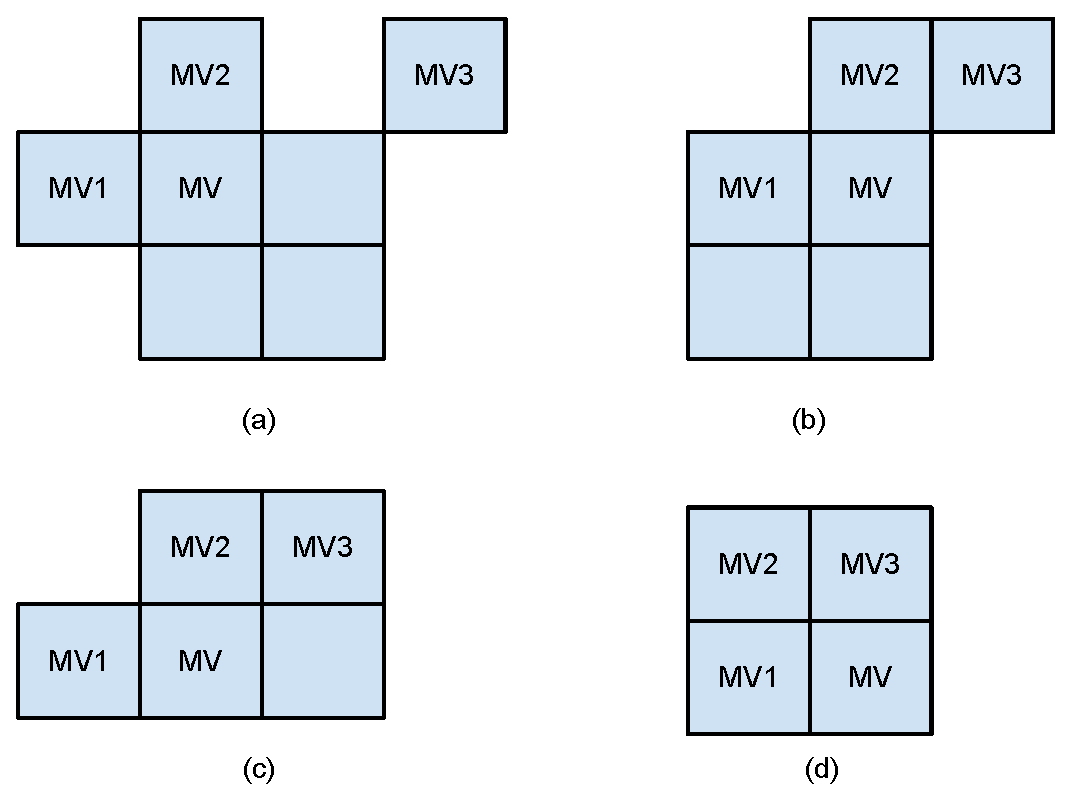
\includegraphics[height=2.5cm]{mv.eps}
\caption{Different Situations of Motion Vector Prediction}
\end{figure}
The positions of the candidate predicators depend on where the current decoding block locates at its macroblock. Note that the MV candicate predicators follow Fig 3(a) for chrominance blocks. 

The MVs are recorded and used directly by decoder so that no MV prediction decoding is needed. Therefore, the dependency due to MV prediction decoding is eliminated completely. There is another reason to save MV values, which is discussed in inter-VOP dependency. 
  
\subsubsection{Inter-VOP Dependency}
Inter-VOP dependency refers to the dependencies among macroblocks at different VOPs. It is caused by motion compensation coding.

In MPEG4 SP, motion compensation decoding only occurs at P-macroblock at P-VOP. Considering the case there is one MV per macroblock, the inter-VOP dependency can be illustrated as below,
\begin{figure}
\centering
%\vspace{2.5cm}
%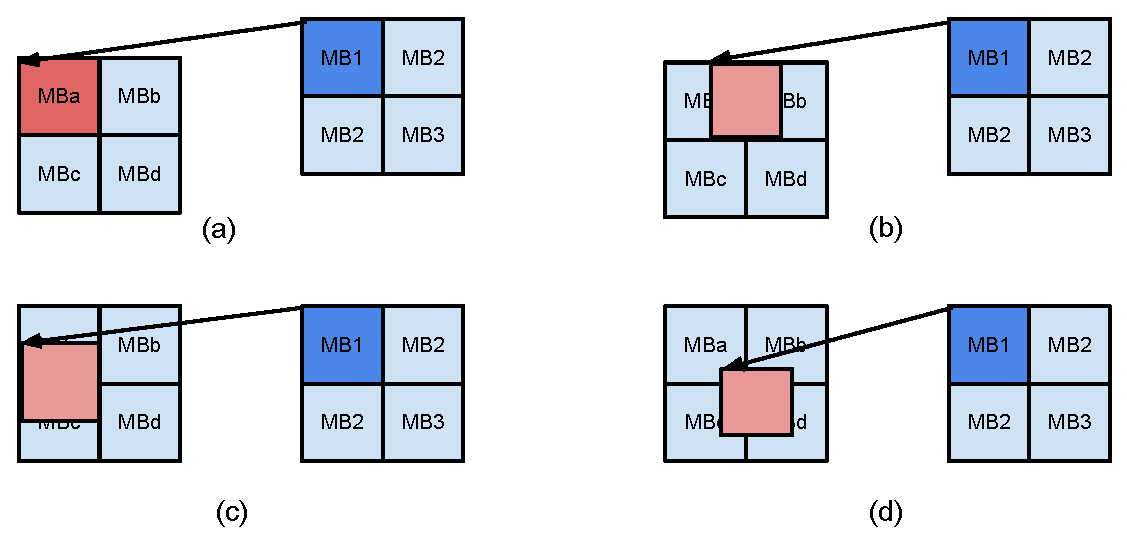
\includegraphics[height=2.5cm]{mm1.eps}
\subfigure[]{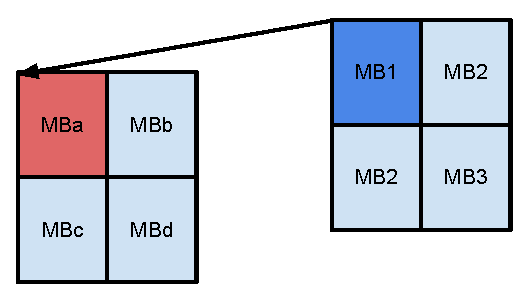
\includegraphics[height=1.5cm]{me1.eps}}
\quad
\subfigure[]{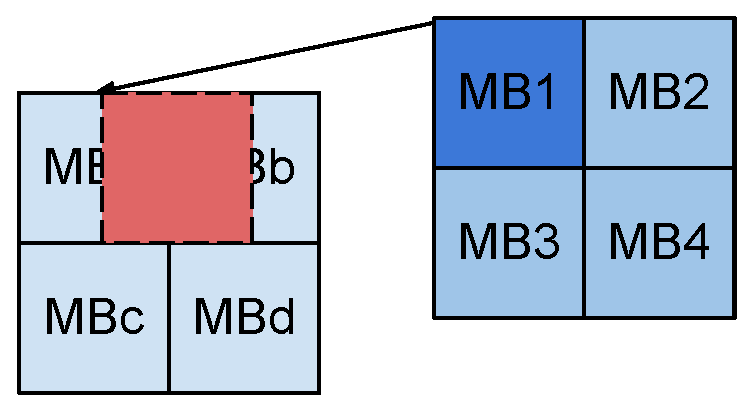
\includegraphics[height=1.5cm]{me2.eps}}
\quad
\subfigure[]{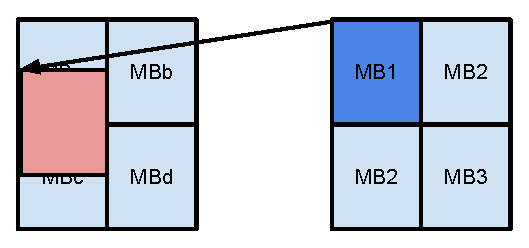
\includegraphics[height=1.15cm]{me3.eps}}
\quad
\subfigure[]{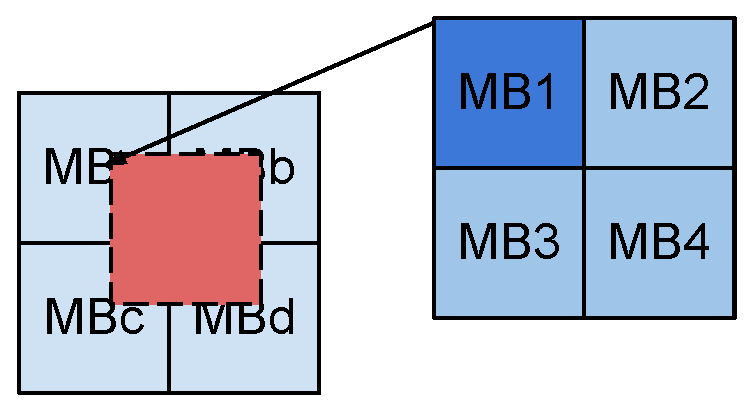
\includegraphics[height=1.15cm]{me4.eps}}
\caption{Different Cases of Motion Compensation Decoding}
\end{figure}
Motion compensation decoding is performed on MB1 of the current frame, with reference to a 16x16 region of a previous frame. Because the reference region does not have to align with the macroblock boundary, the number of dependent macroblocks differ at different cases shown above. At Fig 4(a), MB1 depends on one macroblock. At (b) and (c), it depends on two macroblocks. And at (d), it depends on four macroblocks. 

Khiem etc. proposed an approach to reduce dependency due to motion compensation\cite{Ngo:2011:AEZ:1943552.1943581}. We adopted their technique in this research. Using the case in Fig 4(d) as an example, this is illustrated as below,
\begin{figure}
\centering
%\vspace{2.5cm}
%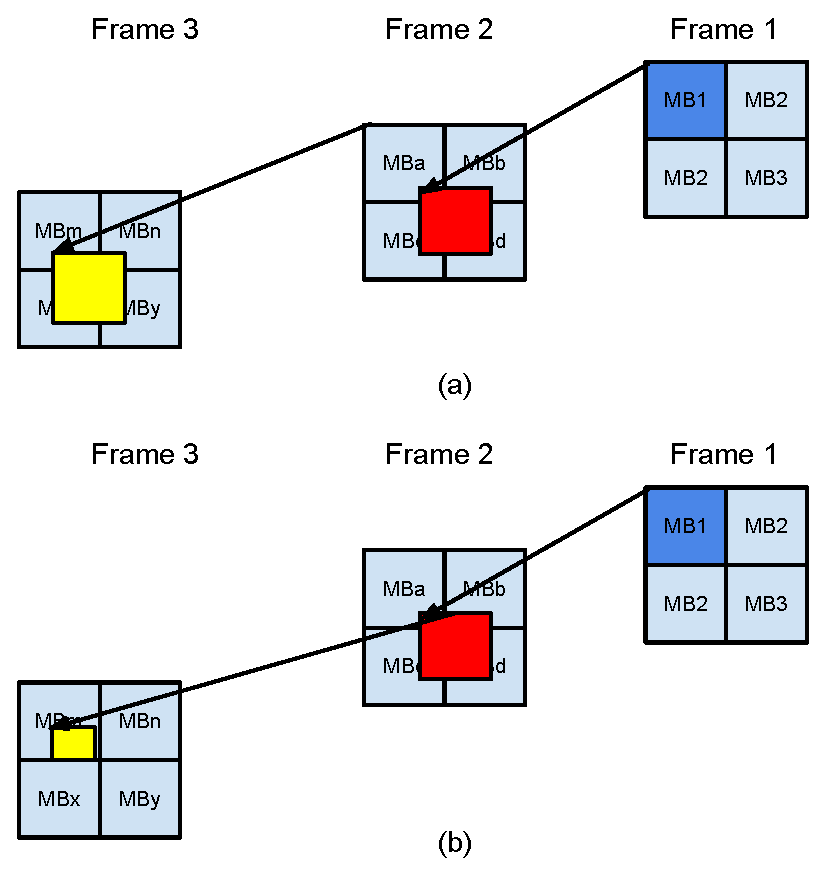
\includegraphics[height=2.5cm]{mm2.eps}
\subfigure[]{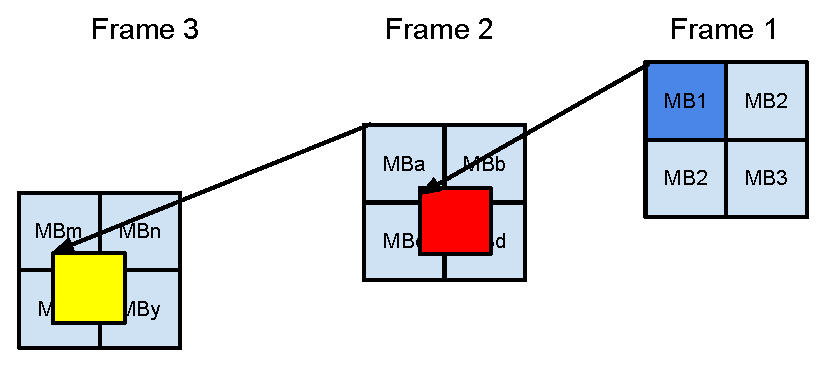
\includegraphics[height=2.0cm]{md1.eps}}
\quad\quad
\subfigure[]{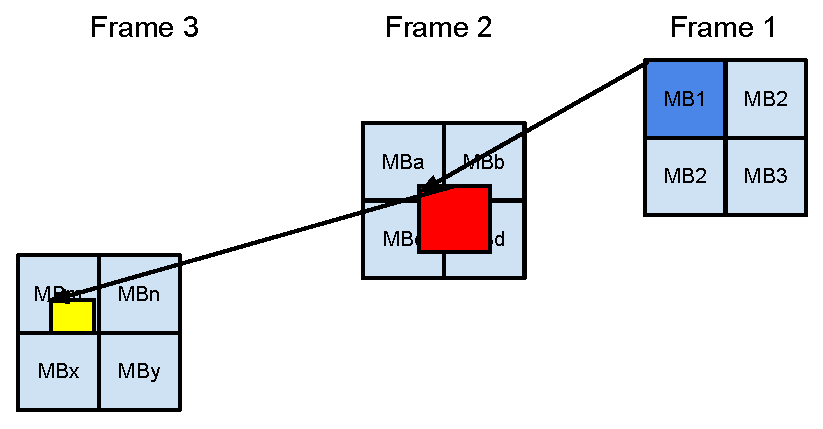
\includegraphics[height=2.0cm]{md2.eps}}
\caption{Dependency Analysis for Motion Compensation}
\end{figure}
To decode MV1 at Frame 1, four macroblocks at Frame 2 are needed. For one of the four macroblocks MBa at Frame 2, another four macroblocks at Frame 3 are needed. Dependency can be reduced by tracing it at pixel level. The dependency between Frame 1 and Frame 2 remains the same. But we do not really need all pixels at Frame 2 MBa. By tracing the dependency at pixel level, the region needed at MBa depends on only part of MBm at Frame 3. Therefore, the dependency for MBa between Frame 2 and 3 are reduced. In the example, it is reduced from four to one for macroblock MBa. 

\subsection{Dependency Files}
The offline computation partially decodes a video and records down the dependency information into a set of files named dependency files. The dependency files are generated for each Group of VOP (GOP). This avoids the issue of dealing with big files when dependency information is stored in a single set of files for the entire video. It also reduces the overhead of switching between files when dependency information is stored on a frame by frame basis. 

For every GOP, the dependency files include the following,
\begin{enumerate}
\item GOP record file: this file contains the start and end frame numbers of a GOP. 
\item MB start position file: this file stores the macroblock start bit position in the video bitstream for every MB of all frames in the GOP. The file is in binary format and each position is stored in four bytes. 
\item MB end position file: this file contains the macroblock end bit position. The start position and end position files are needed for the decoder to seek the bits for a macroblock. 
\item DC\&AC Prediction direction file: this file contains the DC\&AC Prediction direction. A single bit is used to store the direction for each block. The direction is read directly by the decoder to avoid decoding the macroblocks used in DC\&AC Prediction reference selection but not in actual prediction decoding. 
\item MV file: this file records the MV values for every macroblock of each P-VOP in the GOP and the number of bits used to encode the MVs. The selective decoder reads the MV values from this file and skip the encoded bits. This file does not only eliminates the MV decoding dependency, but also allows the online computation to trace the inter-VOP dependency. The file is in binary format.
\item Intra frame dependency file: this file contains the positions of macroblocks that a macroblock directly depends on when only intra-frame dependency is considered. Since MV dependency is eliminated, the only source for intra-VOP dependency is DC\&AC prediction decoding. Note that it is possible to compute this information online based on DC\&AC Prediction direction file, but we obtain this information at offline computation for simplicity. The file is in binary format. 
\end{enumerate}
We modified the standard MPEG4 SP decoder to partially decode a video in order to generate the above files. 

 



